\pr (2b) Vyberte funkciu, ktorej definičný obor je znázornený na obrázku.

\begin{multicols}{2}
\noindent
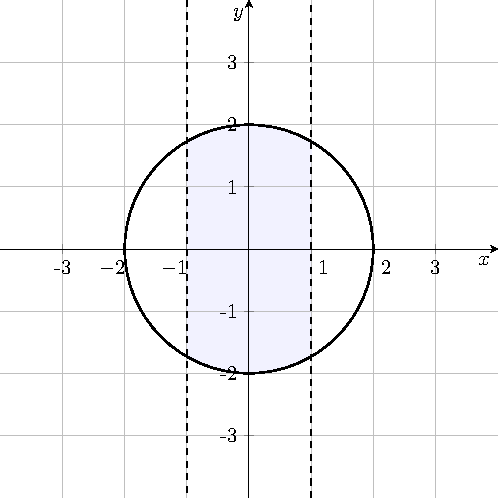
\includegraphics{kruznica1.pdf}

\noindent
\begin{itemize}
\item[a)] $\displaystyle f(x,y)= \arcsin x + \sqrt{4 - x^2-y^2}$
\item[b)] $\displaystyle f(x,y)= \frac{\arcsin x}{\sqrt{4-x^2-y^2}}$
\item[c)] $\displaystyle f(x,y)= \frac{\ln(1-x^2)}{\sqrt{4-x^2-y^2}}$
\item[d)] $\displaystyle f(x,y)= \ln\left(\frac{x+1}{x-1}\right)+\sqrt{4-x^2-y^2}$
\end{itemize}
\end{multicols}
